
As morphisms in $\LREL$ correspond to tropical linear functions, morphisms in the coKleisli category $\LREL_{!}$ 
correspond to a generalization of tropical Laurent series, i.e.~the tropicalization of power series. 
The study of power series in tropical mathematics is very recent (see e.g.~\cite{Porzio2021}) and many properties of these functions still have to be well-understood. 

In this section we recall some known facts about tropical Laurent series, and we establish some new properties, this way highlighting the rich and interesting topological and metric structure of the category $\LREL_{!}$.

%
%In this section we study the tropical Laurent series $\Lawv^X\to \Lawv ^Y$ from the viewpoint of analysis.

\subsection{From tropical polynomials to tLs}

A tropical polynomial, as we saw, is a piece-wise linear function of the form $f(x)=\min_{i_{1},\dots, i_{k}}\{i_{j}x+c_{i_{j}}\}$. For instance, the polynomials $\varphi_{n}(x)=\min_{i\leq n}\{in+2^{-i}\}$
are plotted in Fig.~\ref{fig:plot1} for $n=2,3,4$.
A \emph{tropical root} of a tropical polynomials $\varphi$ is a point $x\in \Lawv$ where $\varphi$ is not differentiable. In other words, the roots of $\varphi$ are the points where the minimum defining $\varphi$ is attained at least twice (i.e.~where the slope of $\varphi$ changes. For instance, the tropical roots of $\varphi_{n+1}$ are of the form $2^{-(i+1)}$, for $i \leq n$.
With this definition, tropical roots mimic the usual factorization property of roots: if $x_{0}$ is a root of $f$, this factorizes as
$f(x)=\min\{x,x_{0}\}+ g(x)$.
%
%A
% simple calculation shows that this condition corresponds, in the tropical setting, to the usual notion of root. 



As anticipated in Section \ref{sectionnew}, a tropical Laurent series (of one variable $x\in\Lawv$), shortly a \emph{tLs}, is a function that can be expressed as $f(x)=\inf_{n}\{nx+\matr f_{n}\}$, with $\matr  f_{n}$ a sequence in $\Lawv$. In other words, a tLs is a ``limit'' of tropical polynomials of higher and higher degree. For instance, the function $\varphi(x):=\inf_{n\in\N}\set{nx+\frac{1}{2^n}}$ (illustrated in Fig.~\ref{fig:plot1}), that we will take as our running example, 
is the ``limit'' of the polynomials $\varphi_{n}$. Since $\inf$s are not in general $\min$s, the behavior of tLS may be less predictable than that of tropical polynomials. For instance, tropical roots for tLs (see \cite{Porzio2021}) may also include limit points.

\begin{figure}
\begin{subfigure}{0.24\textwidth}
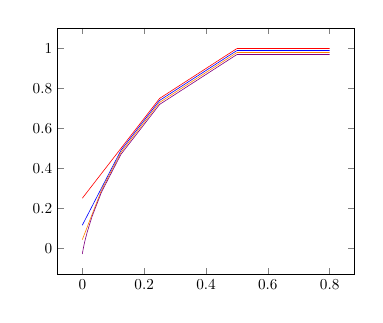
\begin{tikzpicture}[scale=0.55]
\begin{axis}[samples=250]
\addplot[red,domain=0:0.8] {min(2*x+1/4, x+1/2, 1)};
\addplot[blue,domain=0:0.8] {min(3*x+1/8,2*x+1/4, x+1/2, 1)-0.01};
\addplot[orange,domain=0:0.8] {min(4*x+1/16,3*x+1/8,2*x+1/4, x+1/2, 1)-0.02};

\addplot[violet,domain=0:0.8] {min(
10*x+1/1424,
9*x+1/712,
8*x+1/356,
7*x+1/128,
6*x+1/64,
5*x+1/32,
4*x+1/16,3*x+1/8,2*x+1/4, x+1/2, 1)-.03};


\end{axis}

\end{tikzpicture}
\caption{}
\label{fig:plot1}
\end{subfigure}
\begin{subfigure}{0.24\textwidth}
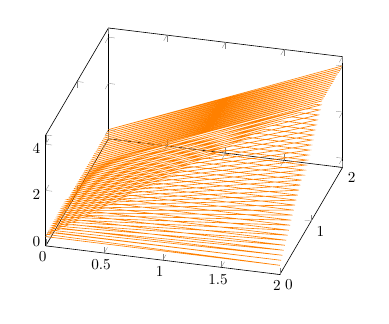
\begin{tikzpicture}[scale=0.55]
\begin{axis}[samples=50, view={15}{45}]
\addplot3[orange,domain=0:2] {min(2*x, 2*x+y, 3*y)};


\end{axis}
\end{tikzpicture}
\caption{}
\label{fig:plot2}
\end{subfigure}
\label{fig:plot12}
\caption{
%\ref{fig:plot1}
 (a) Plot of the tropical polynomials $\varphi_{2}$ (in red), $\varphi_{3}$ (in blue), $\varphi_{4}$ (in orange) and of their limit tLs $\varphi$ (in violet). The points where the slope changes are  the tropical roots of $\varphi$, i.e.~the points $x=2^{-(i+1)}$, satisfying $ix+2^{-i}=(i+1)x+2^{-(i+1)}$.
%\ref{fig:plot2}
(b) Plot of
$\varphi(x,y)=\min\{2x, 2x+y,3y\}$.}
\end{figure} 

%
%
%We will take as our running example
%%given respectively by Equation~\ref{eq:polytrop} and Equation~\ref{eq:defTLS}.
%A positive $x\in[0,\infty)$ is said to be a (finite) \emph{tropical root} of a tropical Laurent series $f:\Lawv\to\Lawv$ iff $f$ is not differentiable at $x$ (w.r.t.\ the usual topology on $\BB R_{\geq0}$.This is equivalent to ask that the $\inf$ defining $f$ at $x$ is obtained \emph{at least} twice.{\color{red} \`e vero anche per TLS o solo per poly questo? Inoltre, Robol parla anche di finite end-points of the domain: nel nostro caso sarebbe $x=0$}

%\begin{example}\label{ex:famous_ex}
% The function $f:\Lawv\to\Lawv$ defined by $f(x):=\inf\limits_{n\in\N}\set{nx+\frac{1}{2^n}}$ is a tropical Laurent series.
%\end{example}

%By plotting its graph {\color{red}vogliamo plottarlo?}, we observe several properties that we will lift to the more general case that we will consider in the next lines, and this example will serve as running one.

%\begin{remark}%[Tropical Laurent series]
 As usual, a matrix $t\in\HOM{\LREL_!}{X}{Y}$ yields a linear map $\Lawv^{!X}\to\Lawv^Y$, but we can also ``express it in the base $X$'', i.e.\ see it as a map $t^!:\Lawv^X\to\Lawv^Y$, by setting 
 $t^!(x):=t\circ_! x$.
%  (we are identifying $\Lawv^X$ with the set $\HOM{\LREL_!}{\emptyset}{X}$ of the \emph{points} of $X$).
 This is the notion of \emph{non-linear} map generated by the CCC-structure of $\LREL_!$.
 Concretely, we have
 \begin{equation}
 t^!(x)_b=\inf\limits_{\mu\in !X} \set{\mu x+ t_{\mu,b}}
 \end{equation}
 where $\mu x:=\sum\limits_{a\in X} \mu(a)x_a$.
 These functions correspond then to tLs with possibly infinitely many variables (in fact, as many as the elements of $X$). %In the following we will also refer to them as tLs. 
 
% 
% We will call them simply \emph{tropical Laurent series (tLs)}.
% %Since in the general case of $\QREL$, $t^!$ is a Laurent series with operations in $Q$, let us call \emph{tropical Laurent series} the functions of shape $t^!$ for some $t\in\HOM{\LREL_!}{X}{Y}$.
%\end{remark}
%
%We find the usual notion of tLs of one variable as follows:

%\begin{remark}
Notice that, by identifying $!\set{*}\simeq \N$ and $\Lawv^{\set{*}}\simeq\Lawv$, the tLs generated by the morphisms in $\HOM{\LREL_!}{\set{*}}{\set{*}}$ are exactly the functions $f:\Lawv\to\Lawv$ of shape $f(x)=\inf\limits_{n\in\N}\set{nx+\matr f(n)}$, for some $\matr f:\N\to\Lawv$, i.e.\ usual tLs's of one variable.
% \end{remark}
 \begin{remark}
 Our running example is indeed of shape $\varphi=t^!$, for $t\in\Lawv^{!\set{*}\times\set{*}}$, $t_{\mu,*}:=2^{-\# \mu}$.
% By Proposition~\ref{prop:descrete}, $f$ is not the interpretation of a $\lam$-term, because its matrix is not discrete.
% Therefore $\LREL_!$ is not a full-complete model of $\STLC$.
\end{remark}



 In a similar way, the tropical polynomials can be identified with the tLs
$f:\Lawv^X\to\Lawv^Y$ 
 for which the support $\C F=\set{\mu\in!X\mid\matr f_{\mu,b}\neq\infty}$ is \emph{finite}, which have thus shape $f(x)_b:=\min\limits_{\mu\in\C F} \set{\mu x+ t_{\mu,b}}$.
 This is again the generalisation of usual tropical polynomials to the case of infinitely many variables.

% 
% , i.e.~for a \emph{finite} set $\C F\subseteq \, !X$.
%%Remark that we also find usual \emph{tropical polynomials} of tropical geometry as a particular case: they 
%correspond to the tLs for which the support $\set{n\in\N\mid\widehat f(n)\neq\infty}$ of $\widehat f$ is \emph{finite}. 
%Actually, for us \emph{tropical polynomial} will mean a function 
%\end{remark}

Looking at Fig~\ref{fig:plot1}, we see that the function $\varphi$, just like the polynomials $\varphi_{1}$, is non-decreasing and concave.
It can be shown that this is indeed always the case:

\begin{proposition}\label{prop:nondecr+conc}
 Any tLs $f:\Lawv^X\to\Lawv^Y$ is non-decreasing and concave, w.r.t.\ the pointwise order.
\end{proposition}

%In Example~\ref{ex:famous_ex}, 
Again, by looking at Fig~\ref{fig:plot1}, it appears that $\varphi$ behaves \emph{locally} like the polynomials $\varphi_{n}$. In particular, for all $\epsilon >0$, $f$ coincides on $[\epsilon,\infty]$ with some polynomial $\varphi_{n}$. Indeed, we can compute  by hand that $\varphi$ coincides with $\varphi_{n}$ 
for $\epsilon \geq \log2/2^{n+1}$.
However, at
%
%$x\in [\epsilon,\infty]$, with $\epsilon>0$
%It can be proven by hand that $\varphi(x)$ is a $\min$ for all $x>0$.
 $x=0$ we have that $\varphi(x=0)=\inf_{n\in\N} \frac{1}{2^n}=0$, and this is the only point where the $\inf$ is \emph{not} a $\min$.
Also, while the derivative of $f$ is bounded on all $\BB R_{>0}$, at $x=0$ it tends to $\infty$.
This phenomenon is reminiscent of [Example 7, \cite{Ehrhard2005}],
%Differentials and Distances in Probabilistic Coherence Spaces. FSCD 2019
which actually motivated our first investigations.
In fact, these properties are shared by all tLs with \emph{finitely} many variables, as shown by the following result.


Remark that $!\set{1,\dots,k}$ can be identified with $\N^k$.
So the matrix of a tLs $f$ with finitely many variables $x=x_1,\dots,x_k$ (and one variable $f(x)$ in output) can be given as a $\matr f:\N^k\to\Lawv$, and $f$ has shape $f(x)=\inf_{n\in \N^k}\set{nx+\matr f(n)}$, where $nx$ is the scalar product.

\begin{theorem}\label{theorem:fepsilon}
 Let $k\in\N$ and $f:\Lawv^k\to\Lawv$ a tLs with matrix $\matr f:\N^k\to\Lawv$.
 For all $0<\epsilon<\infty$, there is a \emph{finite} $\C F_\epsilon \subseteq \N^k$ such that 
% 
% \begin{enumerate}
%  \item If $\C F_\epsilon=\emptyset$ then $f=\infty$ on all $\Lawv^k$;
%  \item If $f(x_0)=\infty$ for some $x_0\in[0,\infty)^k$, then $\C F_\epsilon=\emptyset$;
  %\item 
$f$ coincides on all $[\epsilon,\infty]^k$ with the tropical {polynomial} $P_\epsilon(x):=\min\limits_{n\in \C F_\epsilon}\set{nx+\matr f(n)}$.
% \end{enumerate}
\end{theorem}
%\begin{proof}
%Call $\leq$ the well-founded pointwise order on $\N^k$.
%Now we can let $\C F_\epsilon:=\set{n\in\N \mid
%\widehat f(n)<\infty \textit{ and } \widehat f(m)> \widehat f(n)+\epsilon \textit{ for all } m<n}$.
%\end{proof}




\subsection{Continuity of tLs}%$\Lawv^{X}$ as a normed cone}

$\Lawv^X$ with the usual $+$ and the usual $\cdot$ is a $\BB R_{\geq0}$-semimodule.
Together with the norm $\norm{\cdot}_\infty$, it can be proved that it is a Scott-complete normed cone.
The normed cone structure induces an order on it, called its \emph{cone order}, by setting:
$x\leq y$ iff $y=x+z$ for some (unique) $z\in\Lawv^X$.
This order makes it a Scott-continuous dcpo.
Furthermore we have:

\begin{proposition}
  Tropical Laurent series $\Lawv^X\to\Lawv^Y$ are Scott-continuous on $\BB R_{>0}^X$, w.r.t.\ the cone orders.
  % on the domain and codomain.
\end{proposition}
The tLs $\varphi$ is continuous on $\BB R_{\geq0}=\Lawv-\set{\infty}$ (w.r.t.\ the usual norm of real numbers).
By considering the usual norm $\norm{x}_\infty:=\sup\limits_{a\in X} \absv{x_a}$ on $\Lawv^X$, we could generalise this property by dropping the case of $x$ having some $0$ coordinate:

\begin{theorem}\label{thm:cont}
 Any tropical Laurent series $f:\Lawv^X\to\Lawv$ is continuous on $\BB R_{>0}^X$, w.r.t.\ to the norm $\norm{\cdot}_\infty$.
\end{theorem}
\begin{proof}
 The result follows after proving that if a real-valued function on a locally convex topological $\BB R$-vector space is, locally around $x$, concave and bounded by a finite constant, then it is continuous at $x$.
\end{proof}


\subsection{Lipschitz-continuity of tLs}%$\Lawv^{X}$ as a metric space.}


The norm $\norm{\cdot}_\infty$ naturally induces a metric $\norm{x-y}_{\infty}$ over the spaces $\Lawv^{X}$. 
A consequence of Theorem~\ref{theorem:fepsilon} is that tLs with finitely many variables are locally Lipschitz on all $\BB R_{>0}$.
In this subsection we will refine and generalise this result.
%
%We will show that tLs satisfy suitable Lipschitz properties  w.r.t.~these metrics. 

Let us first look at tropical linear functions:


\begin{proposition}\label{prop:troplinear}
All tropical linear functions $f: \Lawv^{X}\to \Lawv^{Y}$ are non-expansive.  
\end{proposition}
%\begin{proof}[Proof sketch]
%Using the fact that $f(\B x)_{b}= \inf_{a\in X}\matr f_{a,b}+\B x_{a}$,
%the problem reduces to checking that $|(\matr f_{a,b}-\B x_{a})- (\matr f_{a,b}-\B y_{a})| = |\B x_{a}-\B y_{a}|\leq \| \B x-\B y\|_{\infty}$.\end{proof}
This result shows that, in analogy with that happens in usual metric semantics, linear programs are interpreted by non-expansive functions. 
%\begin{proof}
%Using $f(\B x)_{b}= \inf_{a\in X}\matr f_{a,b}+\B x_{a}$,
%first observe that $|(\matr f_{a,b}-\B x_{a})- (\matr f_{a,b}-\B y_{a})| = |\B x_{a}-\B y_{a}|\leq \| \B x-\B y\|_{\infty}$; we now have
%$|f(\B x)_{b}-f(\B y)_{b}| \leq |(\inf_{a\in X}\matr f_{a,b}-\B x_{a})-(\inf_{a\in X}\matr f_{a,b}-\B y_{a})| \leq
%\sup_{a\in X}|(\matr f_{a,b}-\B x_{a})- (\matr f_{a,b}-\B y_{a})|\leq 
% \| \B x-\B y\|_{\infty}$.
%\end{proof}

Before looking at what happens in the case of non-linear programs, let us make the metric structure of $\LREL$ explicit. 
The following proposition provides a useful characterization of the functional metrics in $\LREL$, relying on 
the bijection between $\HOM{\LREL}{X}{Y}$ and set of tropical linear functions from $\Lawv^{X}$ to $\Lawv^{Y}$.
\begin{proposition}
For all tropical linear functions $f,g:\Lawv^{X}\to \Lawv^{Y}$, $\norm{ \matr f-\matr g}_{\infty} =  \sup_{\B x\in \Lawv^{X}}
\norm{ f(\B x)-g(\B x)}_{\infty}$.\end{proposition}

Let us now consider the case of bounded exponentials:
\begin{proposition}\label{prop:boundedlip}
If a tLs $f: \Lawv^{X}\to \Lawv^{Y}$ arises from a matrix $\matr f:!_{n}X\times Y\to \Lawv$, then $f$ is $n$-Lipschitz-continuous.
\end{proposition}
\begin{proof}[Proof sketch]
This follows from Proposition \ref{prop:troplinear} and the remark that, for all $x\in \Lawv^{X}$, $\norm{ !_{n} x-!_{n} y}_{\infty}\leq n\cdot \norm{ x- y}_{\infty}$, where $!_{n} x$ is the restriction of $! x$ to $\C M_{\leq n}(X)$.%
%Using the fact that $f(\B x)_{b}=\inf_{\mu\in \C M_{\leq n}(X)}\{ \matr f_{\mu,b}+ \mu (!_{n}\B x) \}$, where $!_{n}\B x\in \Lawv^{\C M_{\leq n}(X)}$ is given by 
%$(!_{n}\B x)_{[a_{1},\dots, a_{k}]}=\sum_{i=1}^{k}\B x_{a_{i}}$, 
%it suffices to check that $\| (!_{n}\B x)-(!_{n}\B y)\|_{\infty}\leq n\cdot \| \B x-\B y\|_{\infty}$ and apply Proposition \ref{prop:troplinear}.
\end{proof}
This result is perfectly analogous to what happens in the metric models discussed in Section \ref{section2}, the bounded exponentials $!_{n}$ playing the role of the re-scaling trick.

We can now look at what happens with tLs, i.e.~when considering the full exponential $!$.
First, since a tropical polynomial can be represented as a tropical linear function from $\Lawv^{\C M_{\mathrm{deg}(\varphi)(X)}}$ to $\Lawv$, from Proposition \ref{prop:boundedlip} we deduce:
\begin{proposition}\label{prop:polylip}
Any tropical polynomial $\varphi:\Lawv^{X}\to\Lawv$ is $\mathrm{deg}(\varphi)$-Lipschitz continuous.
\end{proposition}

The proposition above, together with Theorem \ref{theorem:fepsilon}, can be used to show that tLs with \emph{finitely many} variables are always \emph{locally} Lipschitz over $(0,\infty)^{X}$. Yet, we can prove a more general statement, covering also the infinitary case.


\begin{theorem}\label{thmTLSlocLip}
 All tropical Laurent series $\Lawv^X\to\Lawv$ are locally Lipschitz on $\BB R_{>0}$.
\end{theorem}
\begin{proof}[Proof sketch]
The core of the proof is a convex analysis argument (see the Appendix) showing that an arbitrary function $f:\Lawv^X\to\Lawv$ which is non-decreasing, concave and continuous, must be locally Lipschitz. 
\end{proof}


The results just presented translate into the following facts about the interpretation of higher-order programs:
\begin{corollary}
For any $\lambda$-term $M$:
\begin{enumerate}
\item if $\Gamma \vdash_{\BSTLC} M:A$, then $\model M:\model\Gamma \to \model A$ is a Lipschitz map.
\item if $\Gamma \vdash_{\STLC}M:A$, then $\model M: \model\Gamma \to \model A$ is a locally Lipschitz map.
\end{enumerate}
\end{corollary} 
\begin{proof}
As we observed, the interpretation $\model A$ of a bounded type is a finite set, hence $\model M$ must be finite  and  its corresponding linear map $\Lawv^{\model A} \to \Lawv^{\model B}$ is thus a tropical polynomial, so we apply Prop.~\ref{prop:polylip}.
Claim 2) follows directly from Theorem~\ref{thmTLSlocLip}.
\end{proof}


Finally, let us discuss the differential structure. The differential operator $D$ of $\LREL_{!}$ translates into a differential operator $D_{!}$ turing a tLs $f:\Lawv^{X}\to \Lawv^{Y}$ into a tLs $D_{!}(f):(\Lawv^{X})^{2}\to \Lawv^{Y}$, linear in its first variable, and given by 
\begin{equation}
D_{!}f(x,y)_{b}=\inf_{a\in X, \mu\in !X}\left\{\matr f_{\mu*a}+x_{a}+\mu y\right\}
\end{equation}
One can check that, when $f$ is a tropical polynomial, $D_{!}f$ coincides with the standard tropical derivative (see e.g.~\cite{Grigoriev2017}).
Moreover, the Taylor formula \eqref{eq:taylorcat} yields 
a Taylor formula for tLs of the form 
$f(x)=\inf_{n}\left\{D_{!}^{(n)}(f)(!_{n}x,\infty)\right\}$.
The following result shows that the distance between two tropical maps can be approximated using the terms appearing in their Taylor expansions:
\begin{proposition}
For all tLs $f,g: \Lawv^{X}\to \Lawv^{Y}$, and for all $n\in \BB N$, 
the functions $x\mapsto D_{!}^{(n)}(f)(!_{n}x,\infty)$ are $n$-Lipschitz. Moreover 
$\norm{ \matr f-\matr g}_{\infty}= \sup_{n} \norm{ {\delta^{(n)}f}- {\delta^{(n)}g}}_{\infty}$, 
where $\delta^{(n)}h$ indicates the matrix of $D_{!}^{(n)}h$.
%where $\delta^{(n)}f:( \Lawv^{X})^{n}\to \Lawv^{X}$ is the tropical linear function $\delta^{(n)}f(\B x_{1},\dots, \B x_{n})=
%(\Der^{(n)}f)(\B x_{1},\dots, \B x_{n}, \infty)$. 
\end{proposition} 


%A consequence of this result is that the distance between two differential programs can always be approximated via bounded programs:
%\begin{corollary}
%For all $\lambda$-terms $M,N: A\to B$ of $\STDLC$, for all $\epsilon >0$, there exists $K\in \BB N$ such that 
%$|\|\model{M}-\model{N}\|_{\infty}- | \| \model{
%\end{corollary}
